\section{Effect of Irradiation on Electrical Sensor Properties}
\label{sec:irradiation}

\subsection{Current-Related Damage Rate}
\label{subsec:irradiation_alpha}

\begin{figure}
	\captionsetup[subfigure]{aboveskip=-1pt,belowskip=-1pt}
	\begin{subfigure}[b]{0.49\textwidth}
		\centering
		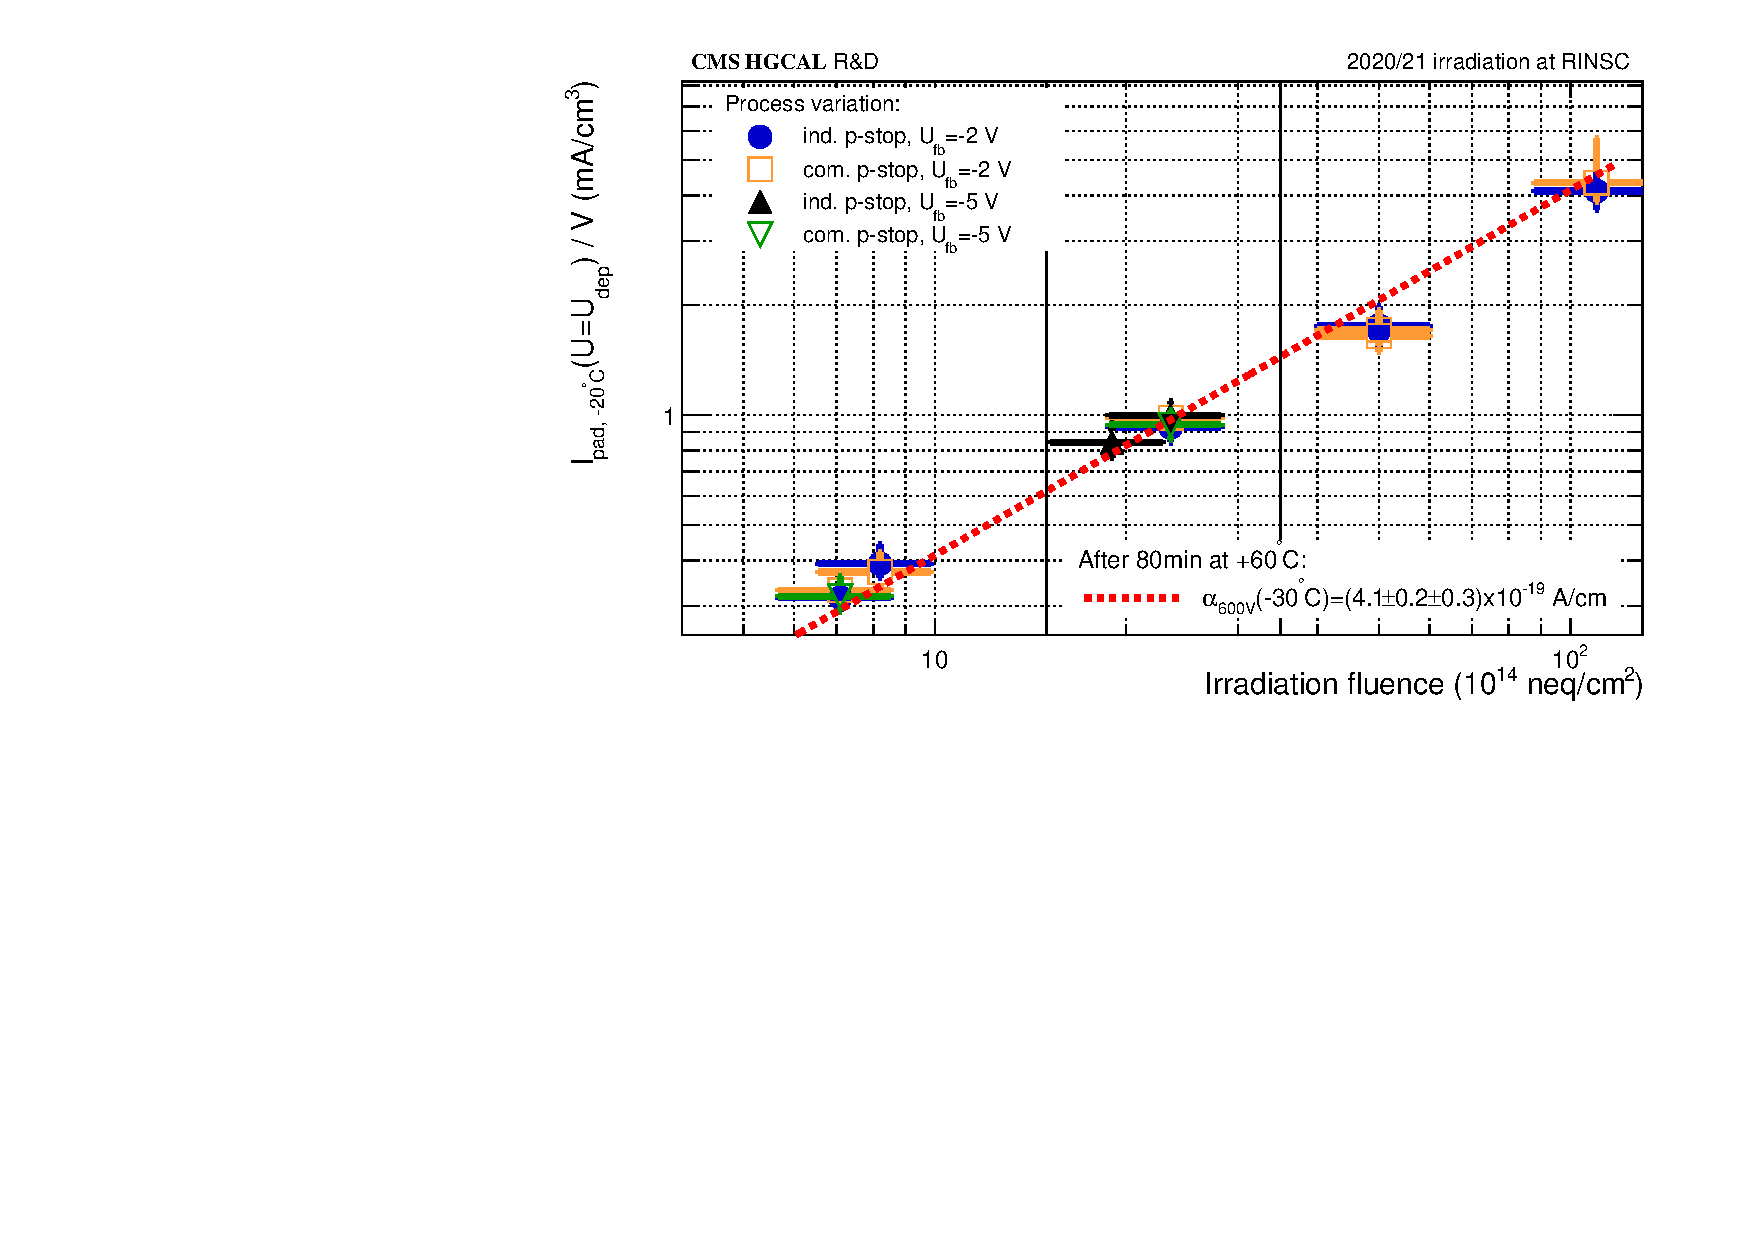
\includegraphics[width=0.99\textwidth]{plots/alpha/alpha_Udep.pdf}
		\subcaption{
			}
			\label{plot:alpha_Udep}
	\end{subfigure}		
	\hfill
	\centering
	\begin{subfigure}[b]{0.49\textwidth}
		\centering
		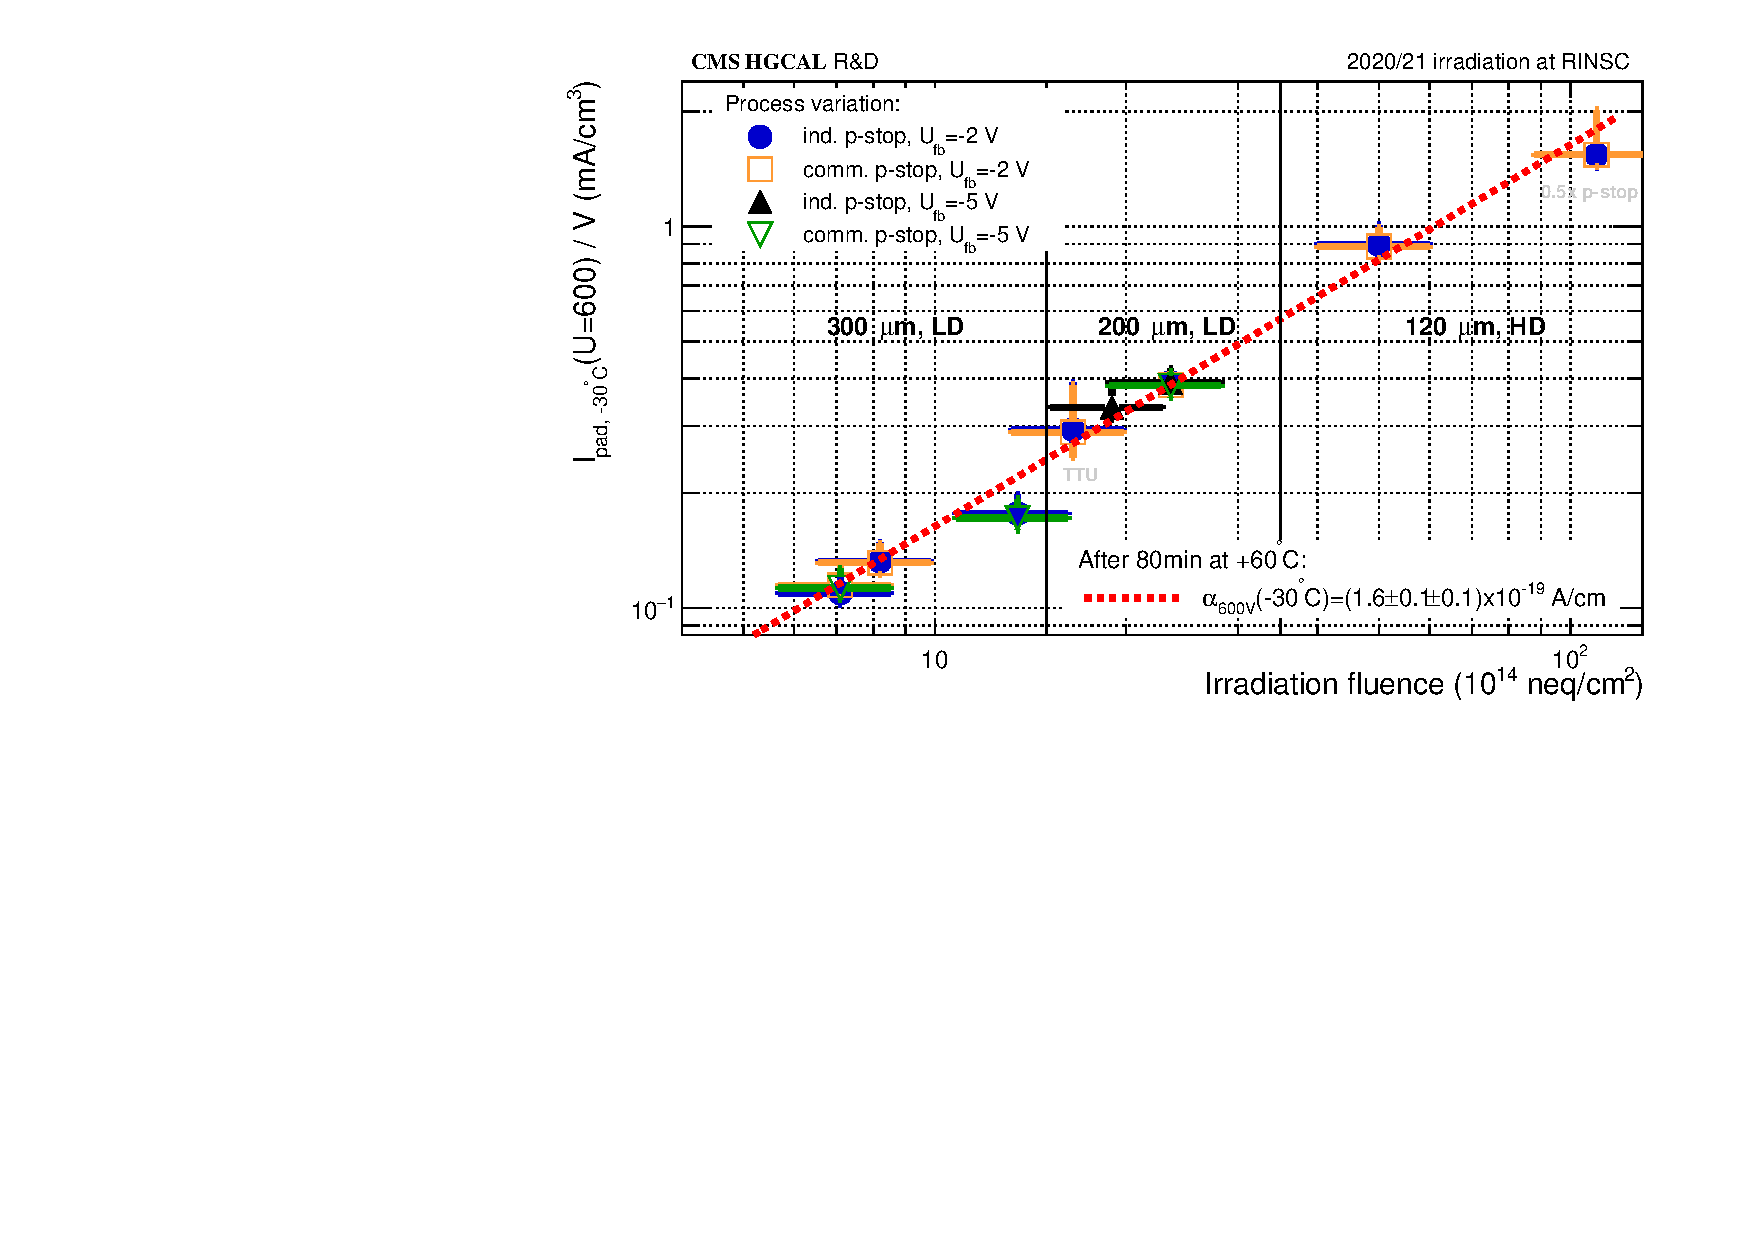
\includegraphics[width=0.99\textwidth]{plots/alpha/alpha_600V.pdf}
		\subcaption{
			}
			\label{plot:alpha_600}
	\end{subfigure}
	\hfill
	\begin{subfigure}[b]{0.49\textwidth}
		\centering
		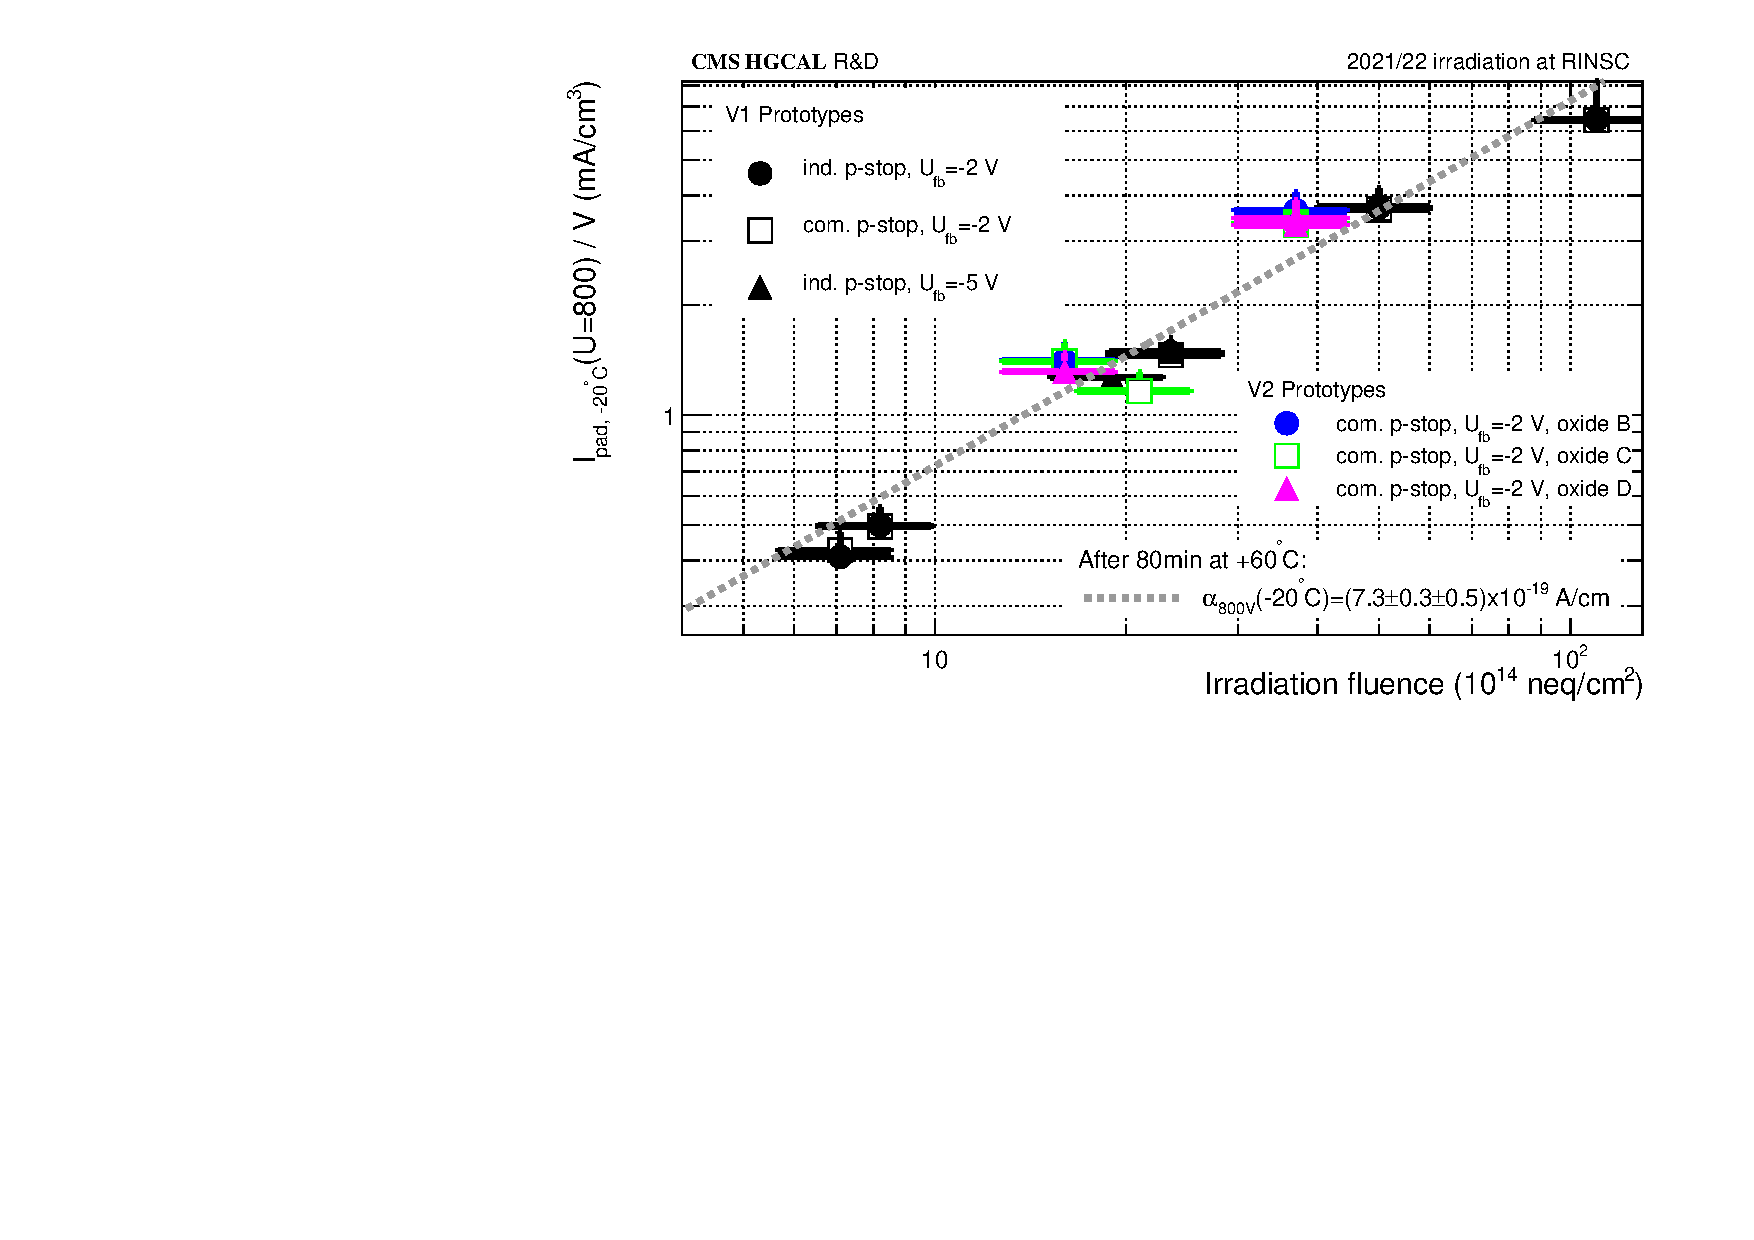
\includegraphics[width=0.99\textwidth]{plots/alpha/alpha_800V.pdf}
		\subcaption{
			}
			\label{plot:alpha_800}
	\end{subfigure}
	\caption{
	    Volume-normalised per-pad leakage current for different fluences at the estimated depletion voltage (a), at a bias voltage of \SI{600}{\volt} (b) and of \SI{800}{\volt} (c).
		Leakage currents were measured after at least \SI{80}{\minute} of additional annnealing at \SI{60}{\celsius}, and were scaled to a temperature of \SI{-20}{\celsius}.
        The current-relate damage rate ($\alpha$) is independent of the sensor production parameters investigated in this work.
	}
\end{figure}

\subsection{Depletion Voltage}

\begin{figure}
	\captionsetup[subfigure]{aboveskip=-1pt,belowskip=-1pt}
	\centering
	\begin{subfigure}[b]{0.49\textwidth}
		\centering
		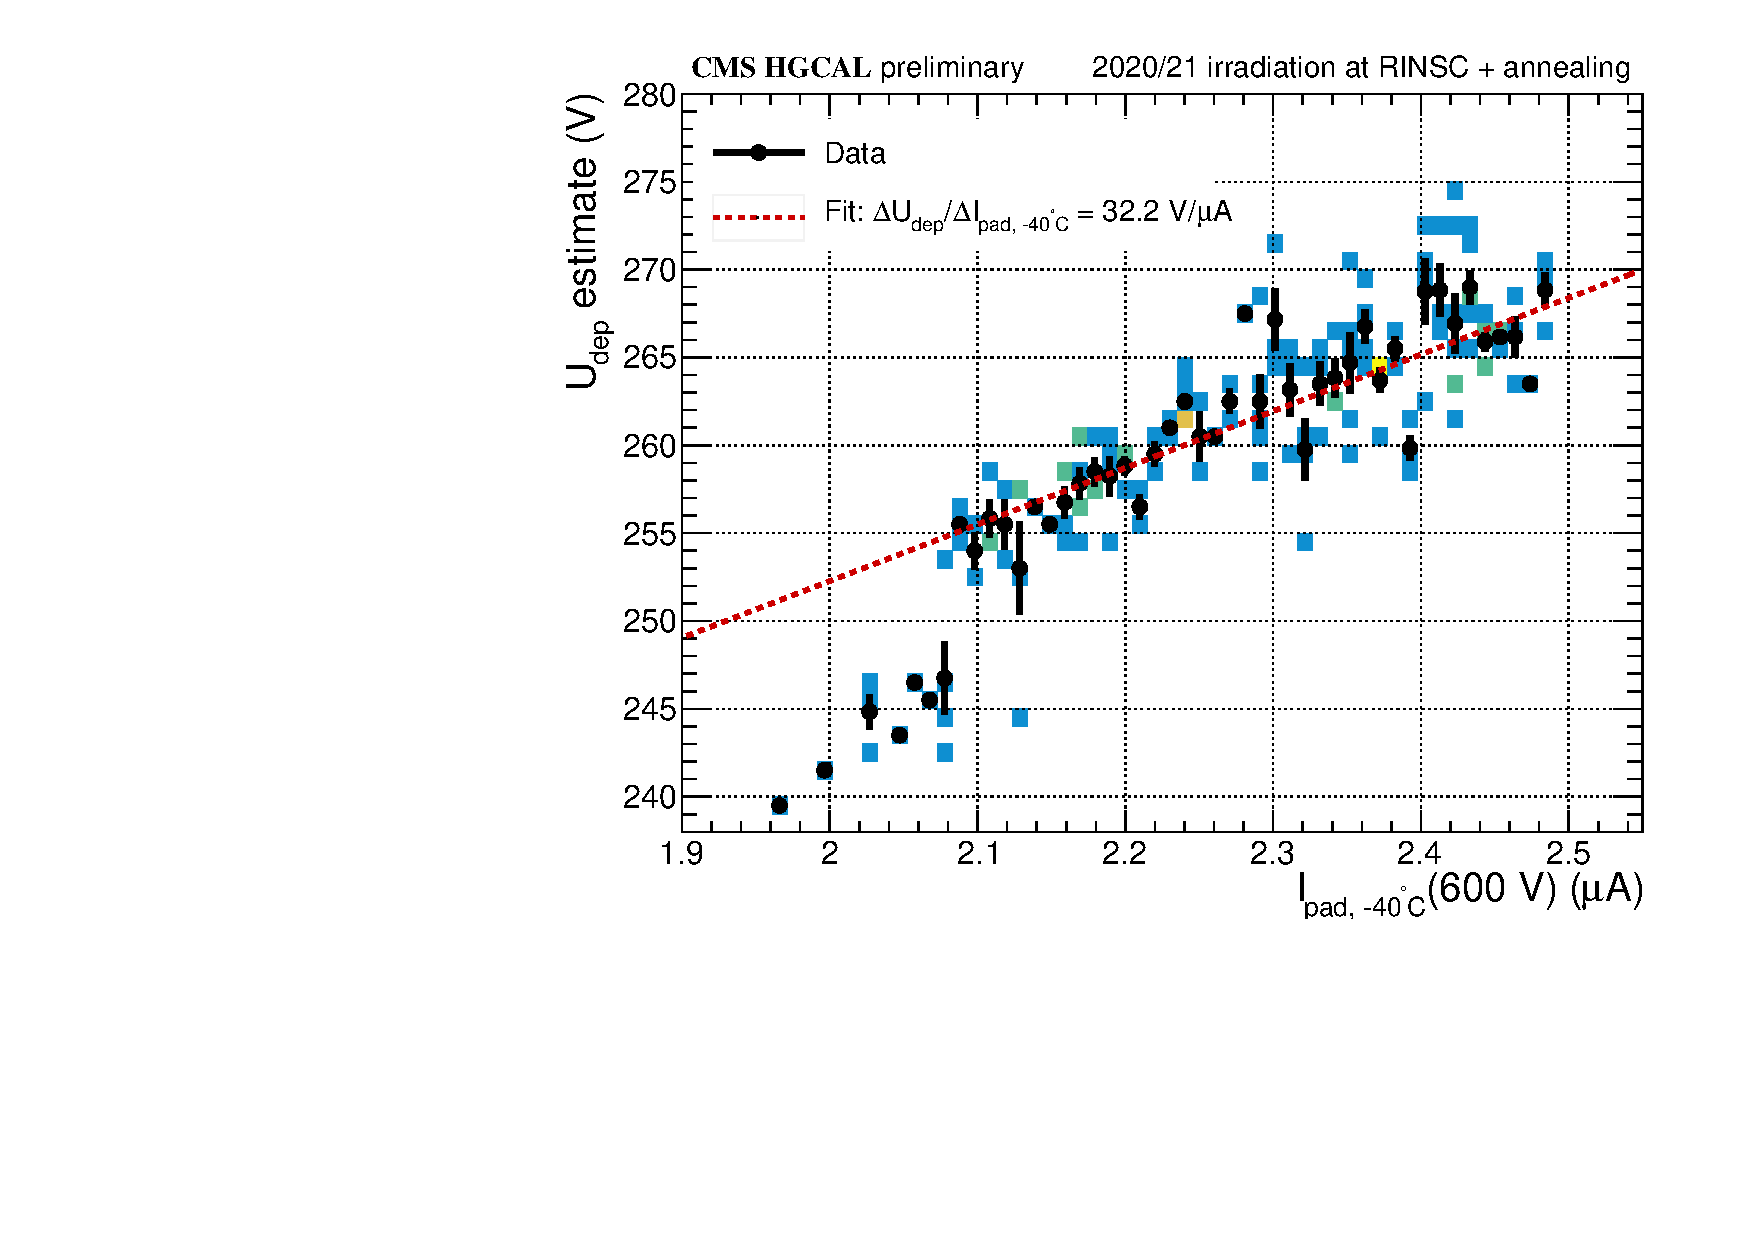
\includegraphics[width=0.999\textwidth]{plots/Vdep_vs_fluence/Vdep_vs_current_5414.pdf}
		\subcaption{
			}
			\label{plot:Vdep_vs_current_5414}
	\end{subfigure}
	\hfill
	\begin{subfigure}[b]{0.49\textwidth}
		\centering
		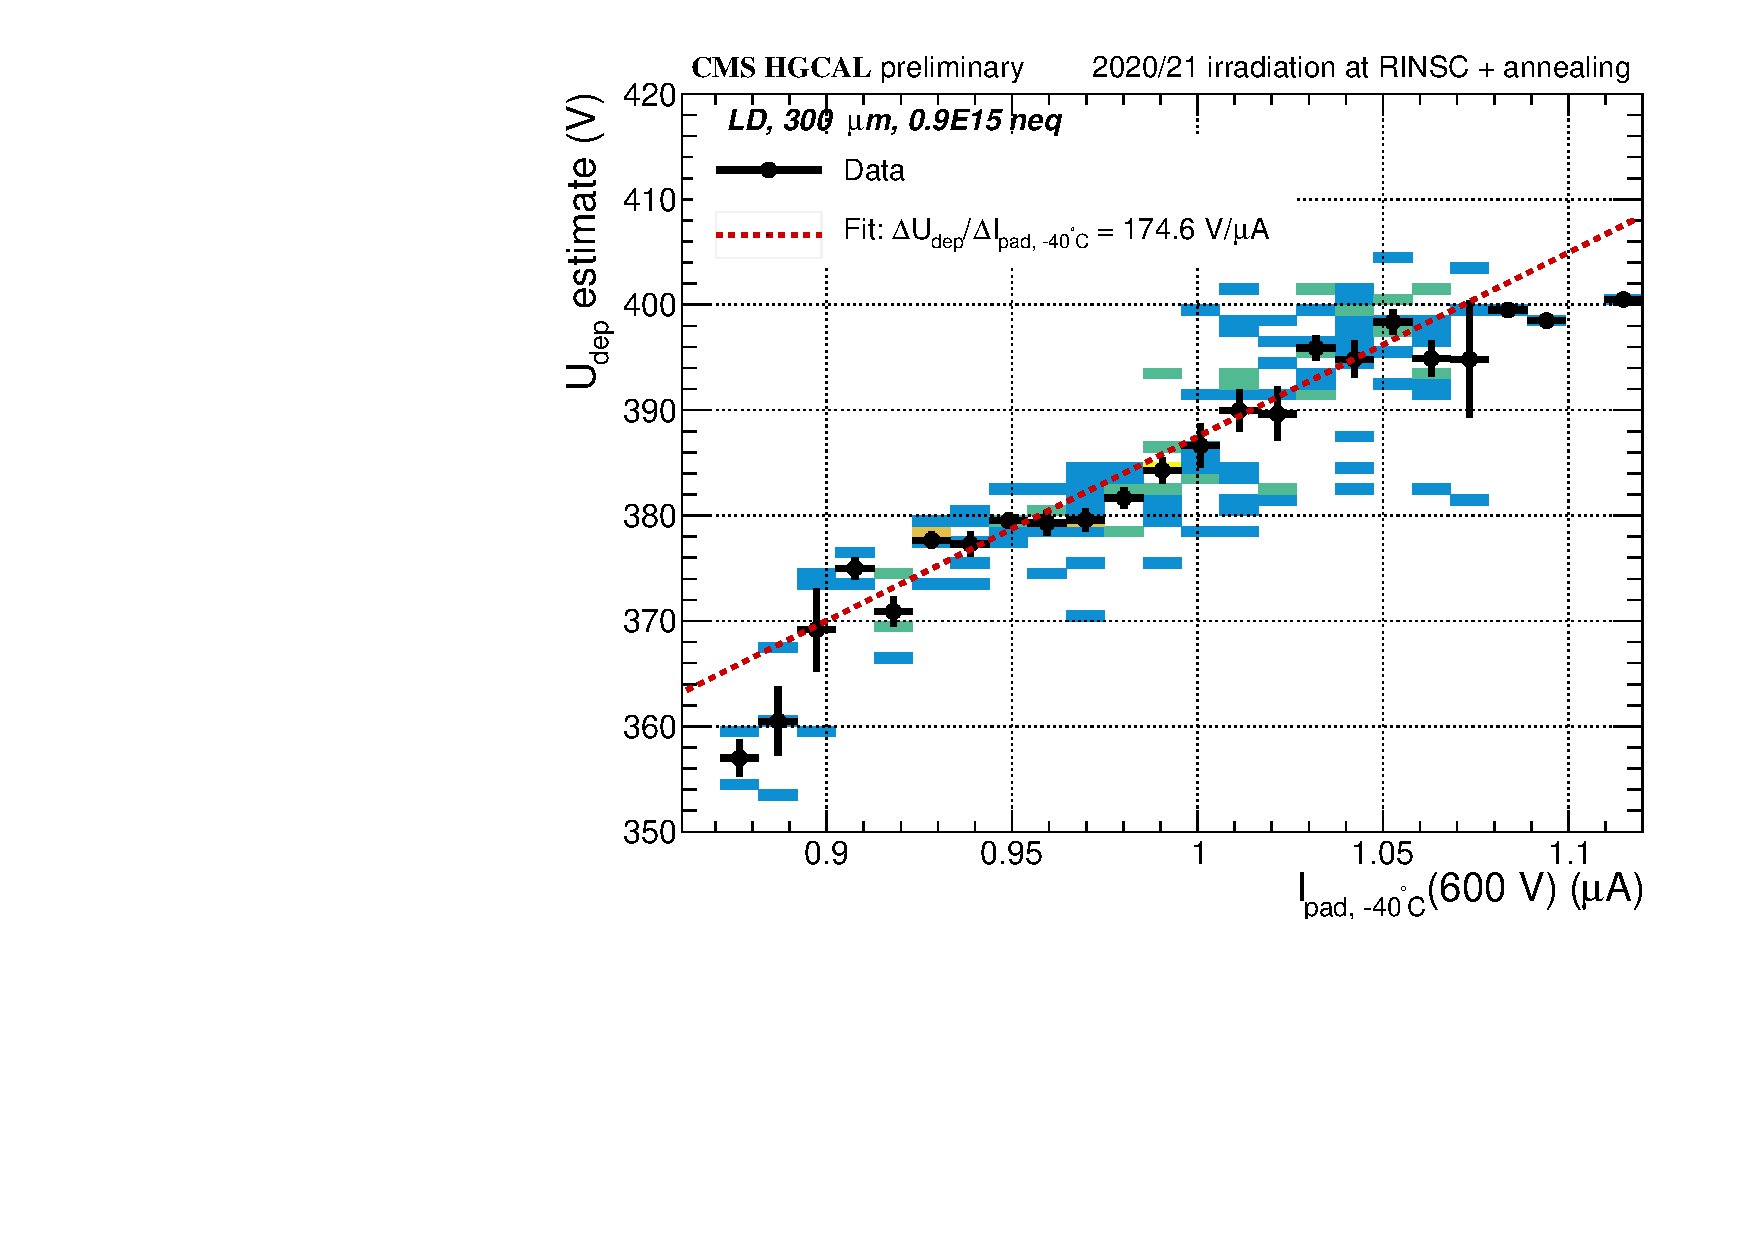
\includegraphics[width=0.999\textwidth]{plots/Vdep_vs_fluence/Vdep_vs_current_1002.pdf}
		\subcaption{
		}
		\label{plot:Vdep_vs_current_1002}
	\end{subfigure}	
	\caption{
		Per-pad depletion voltage estimates vs. per-pad leakage current as proxy for the fluence.
	}
\end{figure}

\label{subsec:irradiation_Vdep}
